\section{Challenges}\label{sec:pcchallenges}



As can be seen in Fig. \ref{fig:caveLight}, the complete absence of natural illumination in combination with the presence of several sources of artificial illumination, such as: each diver's primary light and also one or more video\hyp lights, results in huge lighting variations in the scene. In particular each diver's primary light generates a tightly focused beam which is constantly moving with the motion of the diver. In Fig. \ref{fig:wireReco}a, there are three divers present: one holding the video light, his tanks visible at the bottom of the image; one traveling with the camera, not visible; and a third one whose DPV is visible at the top of the image. The primary light of the third diver can be seen as a blue beam pointing downwards, starting at the left of the DPV. 

\begin{figure*}[p]
	\begin{center}
		\leavevmode
		\begin{tabular}{ccc}
			\subfloat[]{\fbox{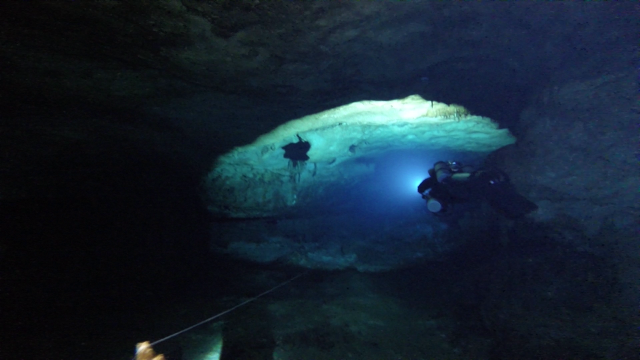
\includegraphics[width=0.62\textwidth]{figures/vlcsnap-2015-04-24-22h02m05s387S}\label{fig:light1}}}\\
			\subfloat[]{\fbox{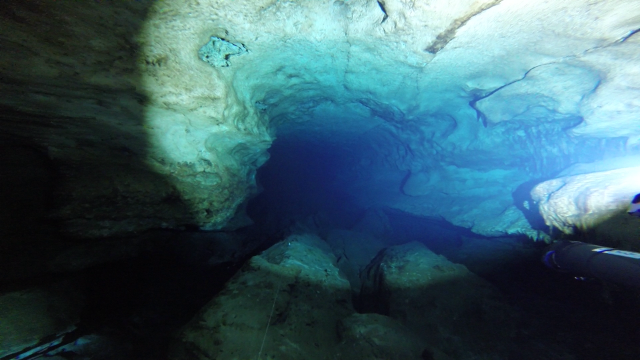
\includegraphics[width=0.62\textwidth]{figures/vlcsnap-2015-04-24-22h04m59s302S}\label{fig:light2}}}\\
			\subfloat[]{\fbox{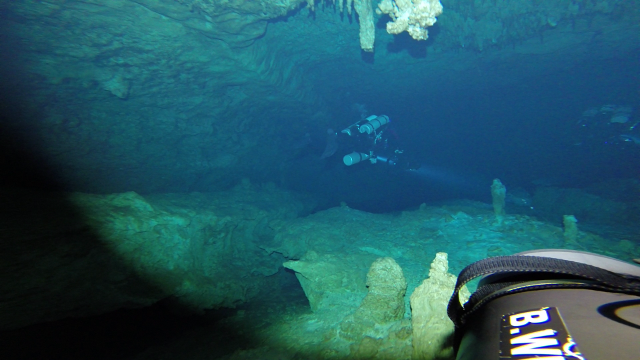
\includegraphics[width=0.62\textwidth]{figures/vlcsnap-2015-04-24-22h09m25s981S}\label{fig:light3}}} 
		\end{tabular}
	\end{center}
	\caption{Left camera images of an underwater cave with different illuminations. Illumination in the cave is provided by the lights individual divers have and also from a strong video\hyp light.  \ref{fig:light1}  Diver in front holds a strong video\hyp light; see how the cone of light outlines the boundaries of the cave. \ref{fig:light2}  Diver with video\hyp light follows behind the camera. \ref{fig:light3} The diver with the camera also holds the light.}
	\label{fig:caveLight}
\end{figure*}

\begin{figure*}[ht]
	\begin{center}
		\leavevmode
		\hspace*{-.2cm}\begin{tabular}{lll}
			\subfloat[]{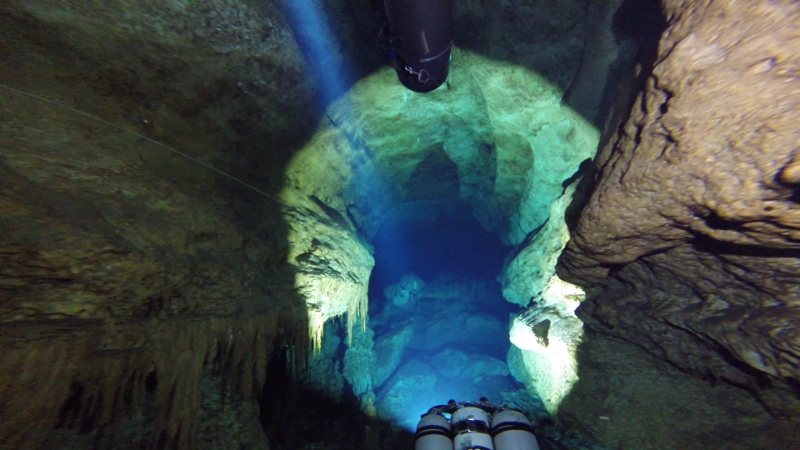
\includegraphics[width=0.47\textwidth]{figures/LUR_0000S}\label{fig:wire1}}&
			\subfloat[]{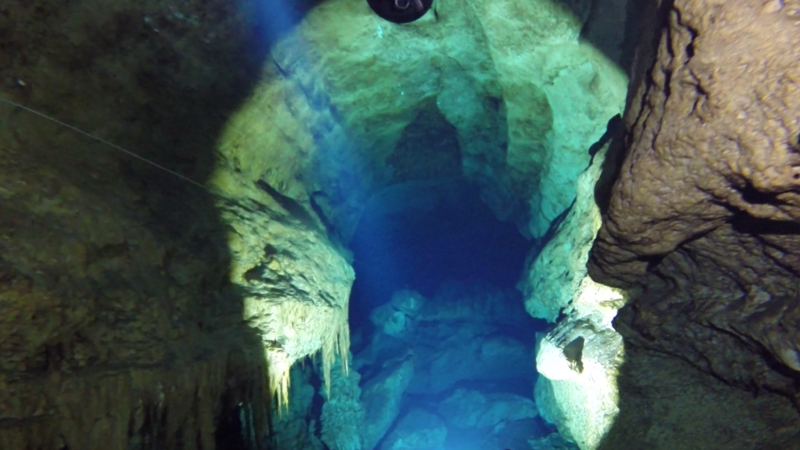
\includegraphics[width=0.47\textwidth]{figures/LR_0000RectS}\label{fig:wire2}}\\
			\subfloat[]{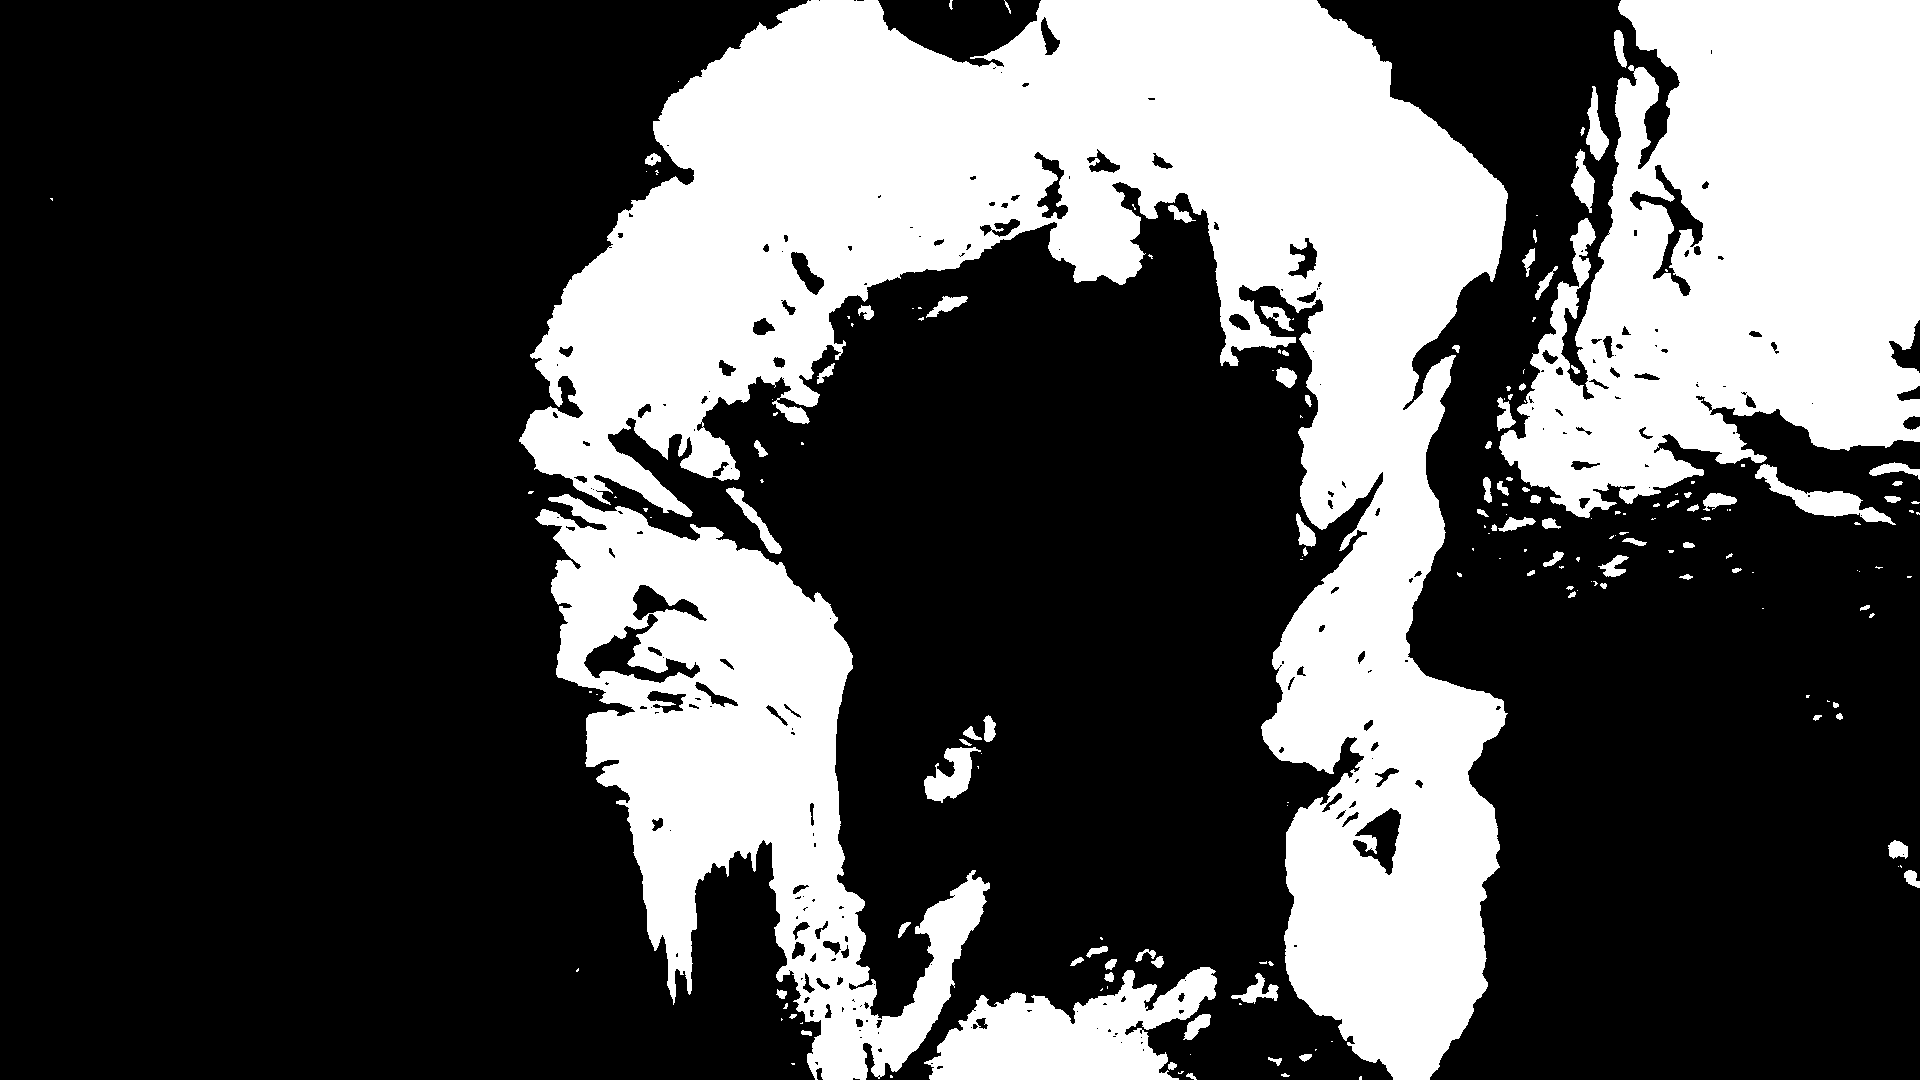
\includegraphics[width=0.47\textwidth]{figures/LT_0000Thr}\label{fig:wire3}}&
			\subfloat[]{\fbox{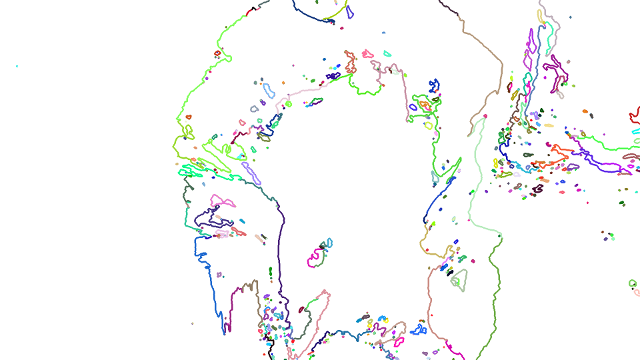
\includegraphics[width=0.47\textwidth]{figures/LT_0000EdgeS}\label{fig:wire4}}}\\
			\subfloat[]{\fbox{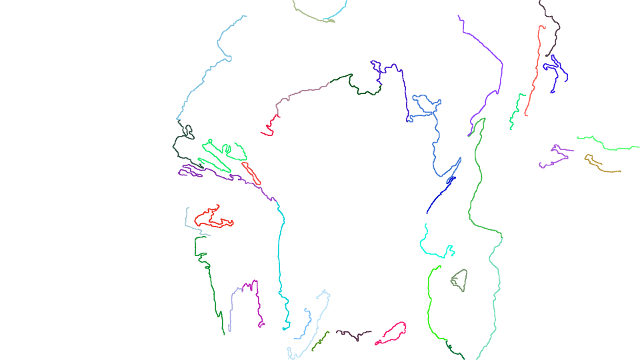
\includegraphics[width=0.47\textwidth]{figures/LT_0000FEdgeS}\label{fig:wire5}}}&
			\subfloat[]{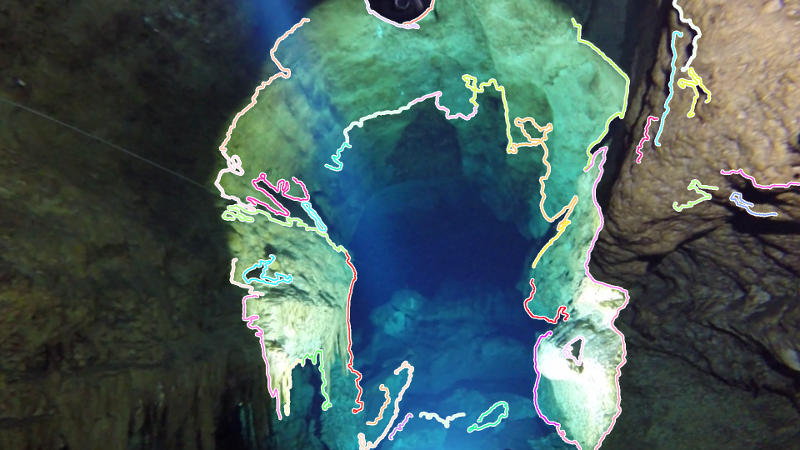
\includegraphics[width=0.485\textwidth]{figures/overlay_with_whiteS}\label{fig:wire6}}
		\end{tabular}
	\end{center}
	\caption{\ref{fig:wire1} Left camera image of an underwater cave.  \ref{fig:wire2} The rectified image. \ref{fig:wire3} The rectified image thresholded based on light intensity. \ref{fig:wire4} An edge map of the boundaries of the thresholded image. \ref{fig:wire5} The boundaries filtered to eliminate small contours. \ref{fig:wire6} The longer contours superimposed on the rectified image.}
	\label{fig:wireReco}
\end{figure*}

The lighting variations make the success of traditional visual odometry~\cite{nister2004visual} algorithms near impossible. The main assumption of Brightness Constancy Constraint underlying most visual odometry algorithms is violated by the constantly moving light\hyp sources. Table \ref{tab1} presents tests of five open source packages of vision based SLAM on underwater cave vision datasets; as expected most of them failed on the longer sequence and the rest were not able to extract the scale of the environment. It is worth noting that several of the packages are expecting specific motions in order to initialize~\cite{klein}. Complete results are not presented due to space constraints; interested readers should refer to the work of Quattrini Li et al.~\cite{RekleitisISERVO2016} for a detailed analysis of more packages and a variety of datasets. The selection of the algorithms presented here was motivated of testing a variety of methods; feature based~\cite{ORB1,4538852}, semi-direct~\cite{forster2014svo}, direct~\cite{raey}, and global~\cite{schoenberger2016sfm}. The main challenge these algorithms face is the constant change of the field of view and the dramatic lighting variations resulting from occlusions and from light absorption over distance. Among the most successful was the ORB\hyp SLAM~\cite{ORB1} with its latest incarnation as ORB\hyp SLAM 2, still in beta version, working with stereo images. While some of these packages, produced an acceptable trajectory, their shape reconstruction was plagued by noise.

%from the detected 3\hyp D features was plagued by noise.

\begin{table*}[htbp]
	\caption{Performance of different open source vision based SLAM packages on underwater data; for a detailed analysis please refer to Quattrini Li et al.~\cite{RekleitisISERVO2016}}
	\resizebox{\columnwidth}{!}{
		\begin{tabular}{|c|c|c|c|c|c|}
			\hline
			&\cite{ORB1}  &  \cite{4538852}&\cite{forster2014svo}  & \cite{raey} &\cite{schoenberger2016sfm}\\
			&ORB-SLAM  & PTAM & SVO & LSD-SLAM & Colmap\\
			\hline
			10 sec & noisy & no initialization & partial trajectories/no scale & loss of track & partial trajectories/no scale \\
			\hline 
			448 sec & noisy & no initialization  & partial trajectories/no scale  & loss of track  & partial trajectories/no scale  \\
			\hline
		\end{tabular}
	}
	\label{tab1}
\end{table*}%
